%author: yjw, 2024-4-1
\subsubsection{ROS2系统机制}
在 ROS 2的体系结构中,节点(Node)是最基本的执行单位,负责特定功能的实现,如数据
处理或硬件接口。每个节点可以包含多种通信机制,包括订阅者(Topic Subscribers)、
定时器(Timer)、服务服务器(Service Servers)和服务客户端(Service Clients),
如图\ref{pic:rns}。这些通信实体的目的是为了接收和发送数据,以及提供不同的服务。

节点注册到执行器(Executor)中,执行器是一个控制实体,负责协调节点的活动。当节点
的一个通信事件发生时,比如收到一个主题消息或服务请求,执行器会调用相应的处理函
数,或称为回调函数(Callback)。这些回调函数是预先定义的,用来响应特定类型的事
件,如 \texttt{topic\_receive()} 用于处理主题消息, \texttt{request\_receive()}
用于处理服务请求,\texttt{time\_up()}用于处理定时器完成计时。

在节点的生命周期中,可以使用生命周期状态机(Lifecycle SM)来管理节点的状态,这在
管理复杂节点时特别有用。生命周期状态机允许节点在不同状态之间转换,如激活
(activate)、去激活(deactivate)和清理(cleanup)。每个状态变化都可以有对应的
回调函数,例如\texttt{setting()}在节点激活时调用,用于声明节点接口、节点执行器
(Executor)、通信订阅和服务订阅等一系列节点功能实体;\texttt{activate()} 用于节
点初始化完毕开始服务,此时节点处于正常工作状态; \texttt{cleanup()}在节点清理资
源时调用,用于释放节点所持有的微机资源。

\textbf{ROS2事件处理机制}: 

节点调用 \texttt{spin()} 函数来持续检查和处理事件,如伪代码\ref{lst:ros_spin}。

\begin{lstlisting}[language=Python, caption=ROS2事件循环示例, label=lst:ros_spin]
spin():
    while True:
        new_msg <- ros_dds_listener()
        handler <- get_callback(new_msg)
        Executor.execute(*handler)
        sleep(0.1)
\end{lstlisting}

\texttt{spin()} 实质是一种事件循环,它会保持节点循环和监听,检查系统中是否有新的
ROS消息或待处理的消息,获取到消息实体后,根据消息类型获取节点初始化时注册的回调
函数,交付给节点执行器去执行,从而完成对该事件(消息)的响应。 \texttt{spin()}函
数是一个事件循环,保持节点持续运行并响应事件。

在执行器内部,\texttt{execute\_any\_*()} 函数是对ROS核心细节的抽象,这个函数根据
事件的类型和优先级选择一个事件来处理。处理过程包括执行注册的回调函数,这些函数是
在节点初始化时注册的,如\texttt{timer.registe\_handler()}用于注册定时器事件的回
调;\texttt{subscriber.regeste\_handler()} 用来注册监听到某话题时触发的回调函
数,以处理该数据。

总体而言,ROS2的程序机制基于事件驱动的模型,通过节点、执行器和回调函数协同工作来
响应和处理各种事件,这些事件可能来源于数据的接收、定时器的触发、服务的请求和响
应,以及节点生命周期状态的变化。通过这种灵活且模块化的设计,ROS 2能够支持复杂且
多样化的机器人系统开发。


\begin{figure}[H]
    \centering
    \includegraphics[width=15cm]{ros_node_setup.png}
    \caption{ROS节点内部模型, 初始阶段}
    \label{pic:rns}
\end{figure}

\textbf{ROS2节点释放}

当ROS2系统的节点将释放时,节点的生命周期状态机会从 activate 状态转换为
deactivate 状态,此状态仅用于让节点完成必要的最后工作,如完成正在处理的数据传输
或请求,然后进入非活跃状态。

紧接着,节点生命周期状态机转为 cleanup 状态,见图\ref{pic:rnc},调用
\texttt{cleanup()} 回调函数来释放节点拥有的资源,这包括所有回调函数(callback
handlers),如和话题订阅、定时器、服务等回调函数。然后清理节点所打开的文件,断开
网络连接,释放ROS2上下文,最终释放内存。

\begin{figure}[H]
    \centering
    \includegraphics[width=15cm]{ros_node_cleanup.png}
    \caption{ROS节点内部模型, 释放阶段}
    \label{pic:rnc}
\end{figure}

\textbf{ROS2通信机制}

为了适应机器人系统中复杂的通信需求,ROS2设计了一套专用的通信模型。其基础为“发
布、订阅“模型,支持节点间的异步数据交换。该机制允许ROS2系统内的节点(Node)独立
地发布(Publish)和订阅(Subscribe)消息,而不需要彼此之间的直接连接或相互了解。
这种设计显著提高了系统的灵活性和扩展性,因为它允许任何数量的发布者和订阅者存在于
同一个话题上,从而实现了高效的多对多通信。

在ROS 2的架构中,每个节点可以根据其功能需求,声明为发布者或订阅者,类似图
\ref{pic:rmp},或同时充当这两种角色。发布者负责生成并发布特定类型的消息到一个命
名的话题上,而订阅者则监听这个话题,接收并处理传入的消息。监听到并处理消息时,使
用的是订阅该话题时传入的回调函数来自动处理,订阅者不必同步阻塞就能等待处理订阅消
息。话题本质上是一个数据通道,它通过唯一的名称标识,确保消息的传递和接收的一致
性。每个话题都与一个明确的消息类型相关联,这个消息类型使用YAML格式定义各字段的静
态变量类型,从而定义了该话题传输数据的结构。

此通信机制的一个核心优点是其异步性,使得发布者和订阅者可以独立地操作,增加了处理
并发消息的能力。此外,由于发布者和订阅者之间的解耦,系统组件可以被设计得更为模块
化,易于开发和维护。例如,在自动驾驶的应用场景中,激光雷达传感器节点可以发布其测
量到的数据到话题 \textbackslash scan,而负责建图和规划路径的节点则通过订阅该话题
来实时获取雷达信息,从而完成最终决策。


\begin{figure}[H]
    \centering
    \includegraphics[width=13cm]{ros_msg_passing.png}
    \caption{ROS话题通信机制}
    \label{pic:rmp}
\end{figure}

\textbf{ROS2 通信机制底层实现}

ROS2通信机制底层实质是使用UDP Socket来进程间通信,使用的协议为物联网DDS协
议,ROS2核心库对其进行了抽象封装,已便捷地被开发者调用。具体而言,对于每种DDS协
议版本,ROS2会实现一种网络中间件对其API进行包装,并实现由ROS2各类消息形式向DDS消
息格式的序列化与结构化转化。如图\ref{pic:rmpm}

\begin{figure}[H]
    \centering
    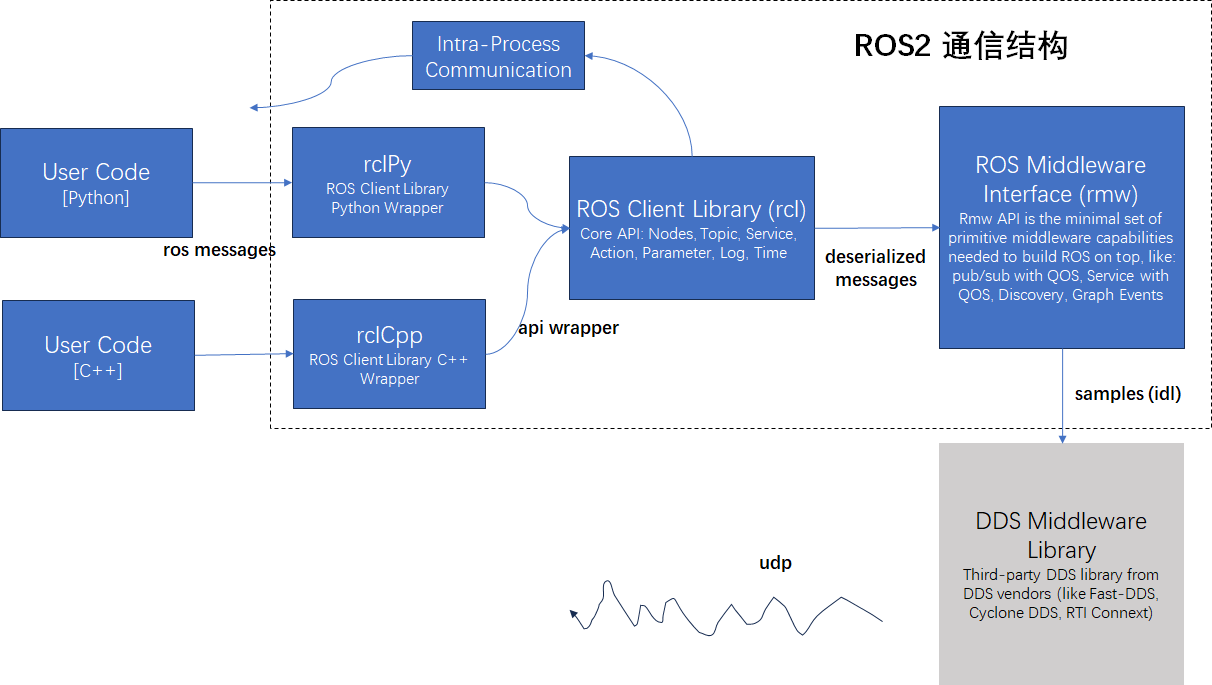
\includegraphics[width=13cm]{ros_msg_passing_mdw.png}
    \caption{ROS底层通信机制实现}
    \label{pic:rmpm}
\end{figure}